\section{Ablations}

\begin{figure*}[tb]
  \centering
  \includegraphics[width=0.99\linewidth]{pics/data_vis.pdf}
  \vspace{-8pt}
  \caption{Subplots illustrate critical properties of \mymethod. (a) Action chunks are projected to 2D via PCA, colored by their assigned primary mode. (b) \mymethod’s one-step MeanFlow decoder achieves FPS comparable to 1-NFE DP3 while maintaining significantly higher success. (c) \mymethod{} preserves high success even with short chunks by avoiding primary mode bouncing.
  }
  \vspace{-16pt}
  \label{fig:data_vis}
\end{figure*}


We perform ablations to quantify the contributions of the two-stage design to study sensitivity to the discrete mode capacity and tokenization, to measure inference-budget trade-offs, and to evaluate how action-chunk length affects success and reactivity.

% \subsection{Primary Mode and MeanFlow Ablation}

\textbf{Primary Mode and MeanFlow Ablation. }We ablate the two core components of our pipeline to establish their individual importance. First is to remove the Mode-conditioned MeanFlow Policy (MF) so that the system simply uses the Primary Mode Policy (PM)’s predicted VQ code and decodes it via the VQ-VAE reconstruction as the final action. Second is to remove the PM so that MF attempts to predict actions without being conditioned on a discrete mode. Results are reported in Table~\ref{tab:ablations}. Removing MF collapses performance almost completely, showing that a raw VQ reconstruction is insufficient as the final action when the number of modes is limited. The quantization error produces large reconstruction distortions that destroy task success. Conversely, removing PM yields a \(0.16\) absolute drop in success, which demonstrates that an explicit primary-mode selection substantially eases the downstream continuous generation problem and prevents coarse-mode bouncing. 

% \subsection{Mode Capacity and Tokenization}

\textbf{Mode Capacity and Tokenization. }We study how the number of discrete primary modes $K$ and the choice of tokenization affect the PM learning and final task performance. We vary $K$ (16, 32, 64, 128) and compare VQ-VAE with a k-means tokenization baseline. Results appear in Table~\ref{tab:ablations}. A smaller $K$ slightly helps the PM to learn, but it risks underfitting when the task’s action-chunk distribution is complex. Larger $K$ increases expressivity but makes the PM harder to learn. In our domains the trade-off is modest and $K=64$ achieves a good balance across tasks. Different tokenizers produce similar final success rates, suggesting the approach is robust to discretization methods. Our method mainly needs a reasonable set of coarse modes rather than a specific quantizer. To further illustrate mode structure we project action-chunks into 2-D (PCA) and color by assigned mode. The visualization shows clear coarse-mode clusters on the action manifold, as visualized in Figure~\ref{fig:data_vis} (a).

\begin{wraptable}{r}{0.45\textwidth}  
  \centering 
  \vspace{-4pt}
  \begin{tabular}{l c c}  
    \toprule  
    Variations & ODE Solver & Success \\ 
    \midrule  
    CFM    & 1-NFE Euler    & \dd{0.69}{0.03} \\
    CFM    & 10-NFE Euler    & \dd{0.69}{0.02} \\
    CFM    & Runge-Kutta    & \dd{0.68}{0.01} \\
    Meanflow    & 1-NFE    & \ddbfgreen{0.72}{0.02} \\
    \bottomrule  
  \end{tabular}
  \vspace{-4pt}
    \caption{Comparison of success for MeanFlow (MF) and Conditional Flow Matching (CFM), varying the ODE solver and NFE.} 
    \vspace{-8pt}
  \label{tab:meanflow}  
\end{wraptable}

% \subsection{Ablation on Meanflow}

\textbf{Ablation on Meanflow. }This ablation aims to evaluate the performance difference between MeanFlow and Conditional Flow Matching (CFM)~\citep{lipman2022flow}, where CFM is tested under different Ordinary Differential Equation(ODE) numerical integration methods. Though CFM theoretically defines a constant velocity field when mapping from noise to target distribution, the parameterized neural network introduces inherent nonlinearity in numerical computations. This makes the exploration of diverse ODE integrators non-trivial. For Runge-Kutta integration, we adopt the Dormand-Prince 5 method, a widely used choice for adaptive-stepsize ODE solving. As shown in Table~\ref{tab:meanflow}, varying ODE numerical integrators yields negligible performance improvements for CFM. In contrast, replacing CFM with MeanFlow results in a consistent performance gain.


% \subsection{Speed–Accuracy Trade-off}

\textbf{Speed–Accuracy Trade-off. }We examine how the number of function evaluations (NFE) during inference affects both inference speed and success. We compare our one-step MeanFlow decoder to DP3 at different NFE settings, plots are in Figure~\ref{fig:data_vis} (b).  Our one-step generator achieves inference speed comparable to DP3 with 1-NFE while delivering substantially higher success. More generally, we observe that within the tested range the total NFE has a surprisingly small influence on success, which suggests that for these simulated tasks the NFE is not the dominant bottleneck. We hypothesize this limited sensitivity is due to the tasks’ tolerance to small action perturbations in simulation. Whether the same holds for very high-precision or contact-sensitive real-world tasks needs further study.

\begin{wrapfigure}{r}{0.6\textwidth}
 % \vspace{-5pt}
  \centering
  % \vspace{-13pt}
  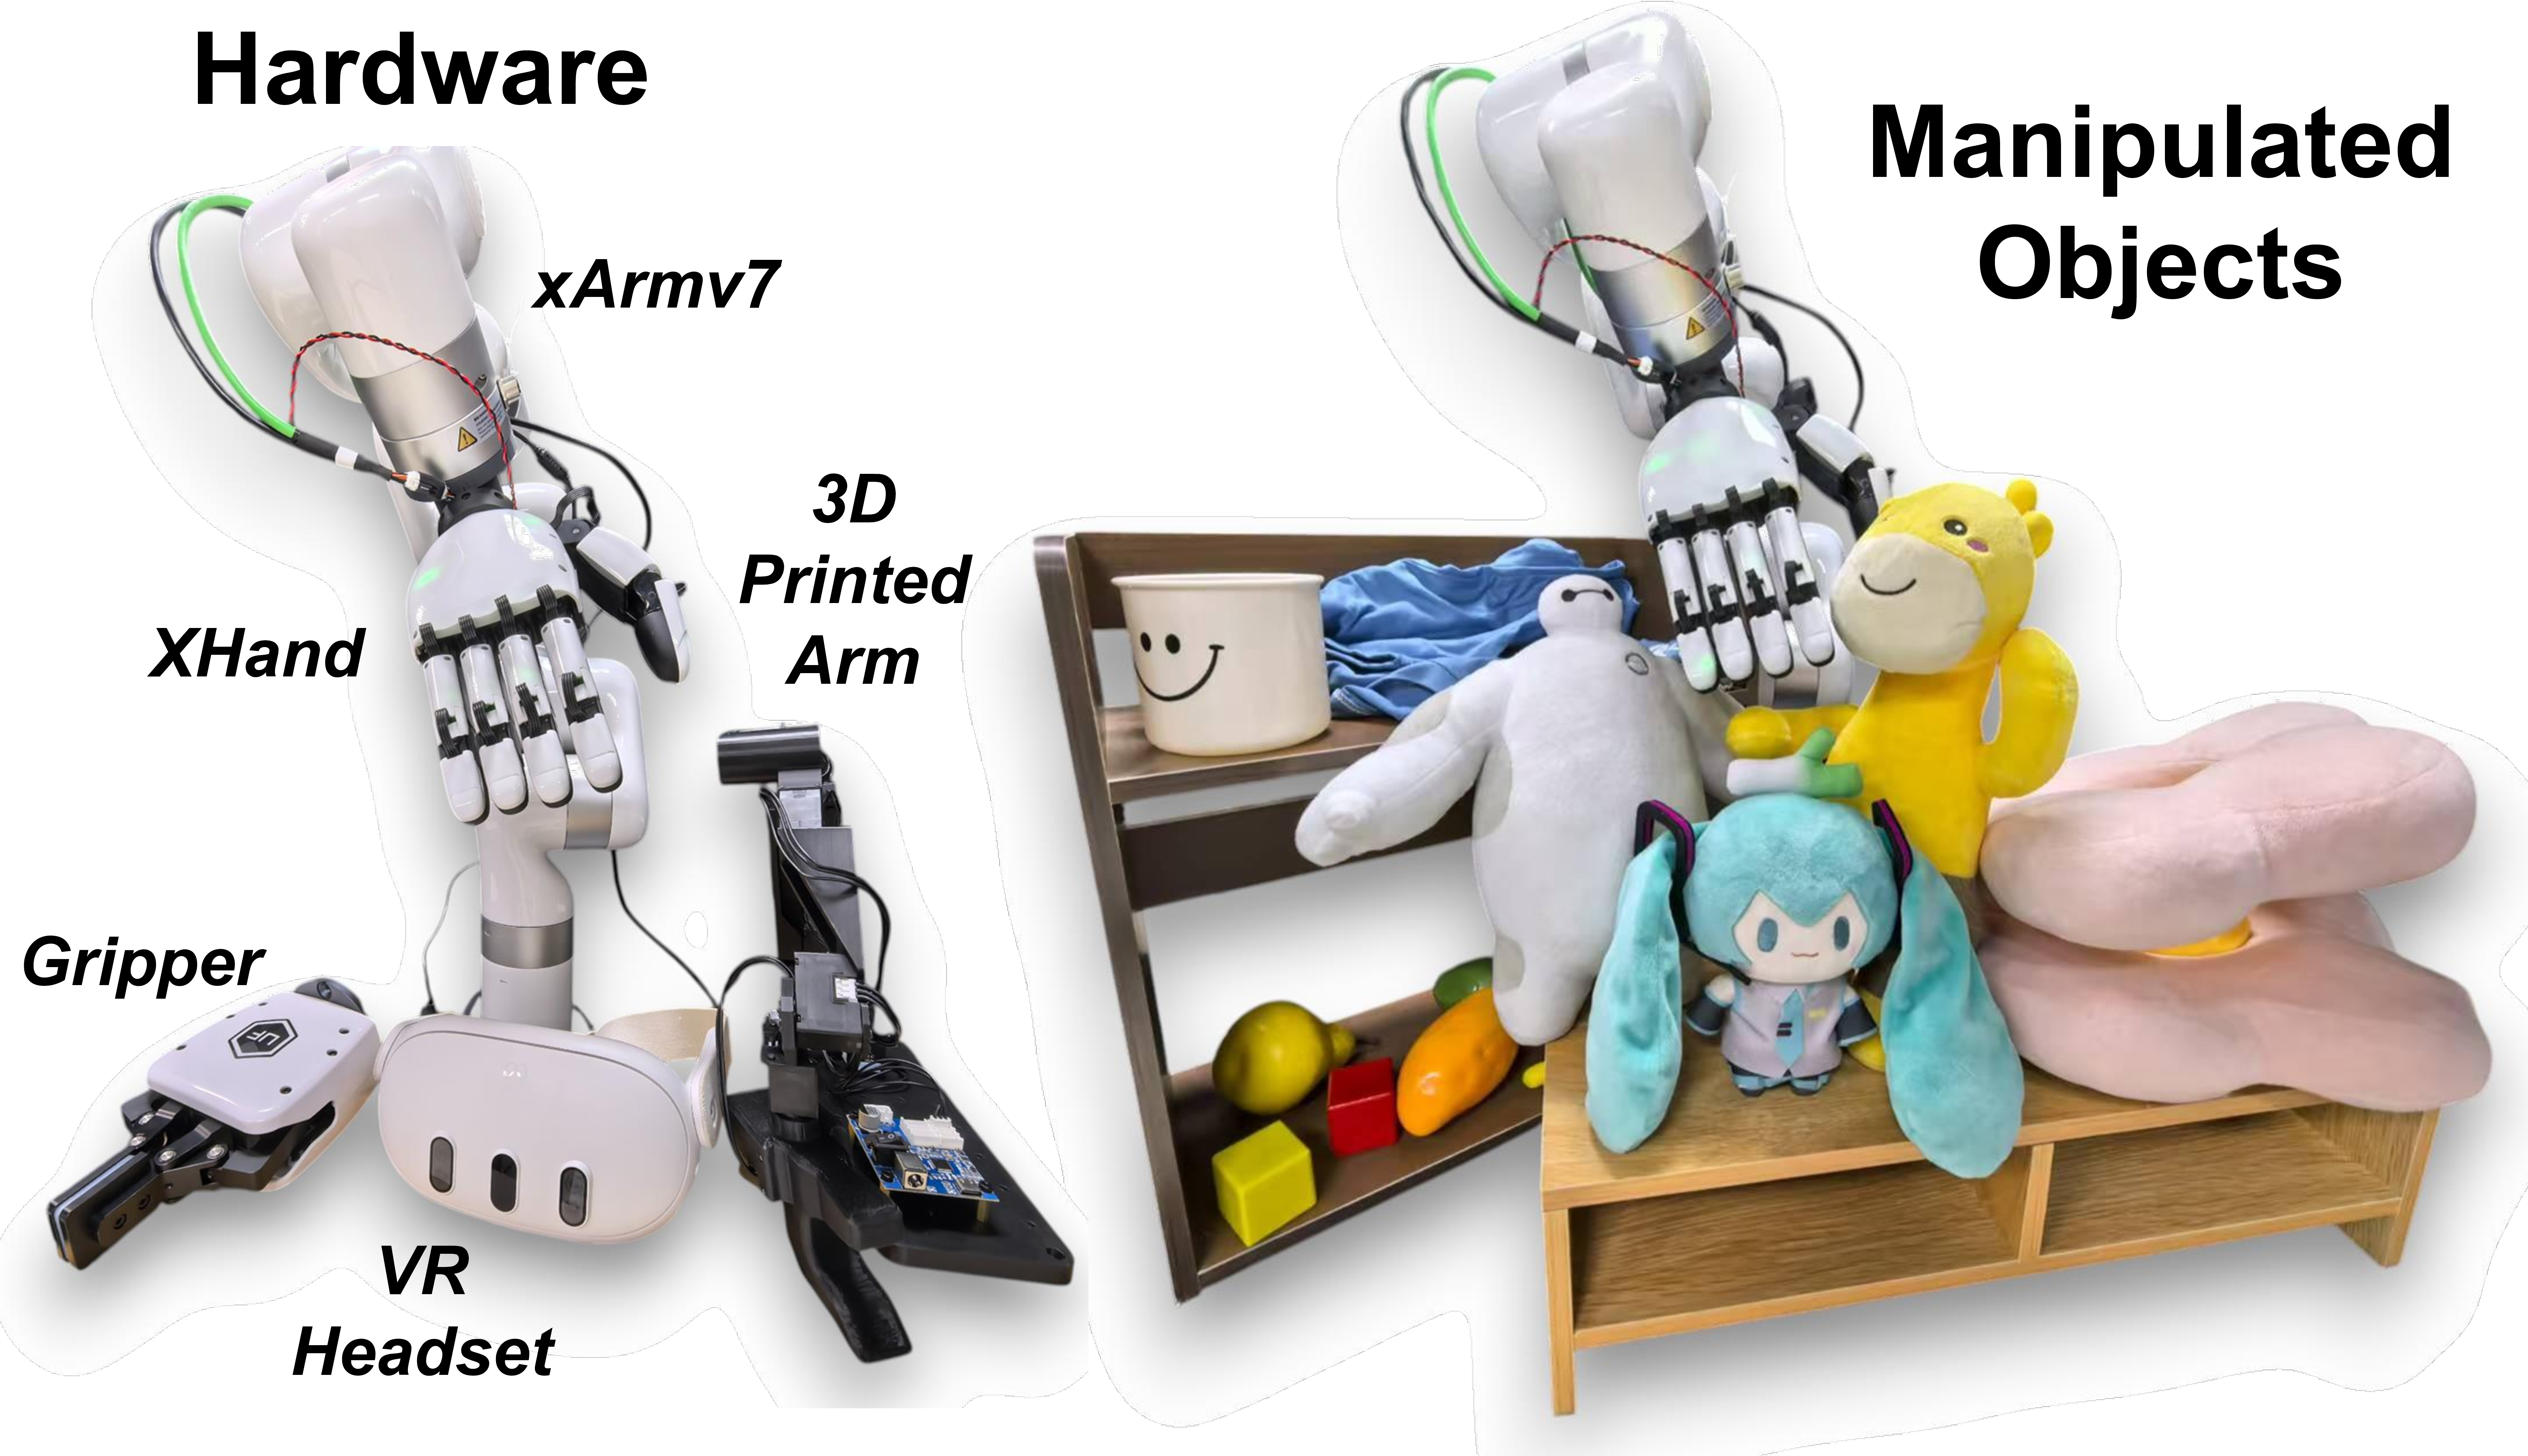
\includegraphics[width=\linewidth]{pics/real_setup.pdf}
  \vspace{-8pt}
  \caption{Hardware and manipulated objects used in real world experiments.}
  \vspace{-16pt}
  \label{fig:real_setup}
\end{wrapfigure}

% \subsection{Action-chunk Length and Reactivity}

\textbf{Action-chunk Length and Reactivity. }All experiments here are conducted on real settings described in the Real World Evaluation section. We sweep action-chunk length and measure success. Shorter chunks make the controller more open-loop reactive and therefore better able to respond to unexpected environment changes. However, short chunks also tend to increase trajectory jitter and occasional stoppages. Our method maintains relatively high success even at short chunk lengths, showing the two-stage design preserves primary-mode consistency while allowing rapid reactivity. Results appear in Figure~\ref{fig:data_vis} (c).



